% Section content template for individual Educative lessons
% This file contains the actual content for a specific section
% Generated from Educative API section content

% Section: System Design: Distributed Monitoring
% Section ID: 6310983387840512
% Section Slug: system-design-distributed-monitoring
% Generated: 2025-12-07T18:13:08.694122

\subsection{Monitoring}\label{GsUGPZa9dS9VlNBagkTU_}
\\
The modern economy depends on the continual operation of IT infrastructure. Such infrastructure contains hardware, distributed services, and network resources. These components are interlinked in such infrastructure, making it challenging to keep everything functioning smoothly and without application downtime.

\begin{figure}[htbp]
 \centering
 
\includegraphics[width=0.25\textwidth]{Images/chapter_13/section_6310983387840512/5685901546881024.png}
 
\end{figure}

It's challenging to know what's happening at the hardware or application level when our infrastructure is distributed across multiple locations and includes many servers. Components can run into failures, response latency overshoot, overloaded or unreachable hardware, and containers running out of resources, among others. Multiple services are running in such an infrastructure, and anything can go awry.\\
\strut \\

\begin{figure}[htbp]
 \centering
 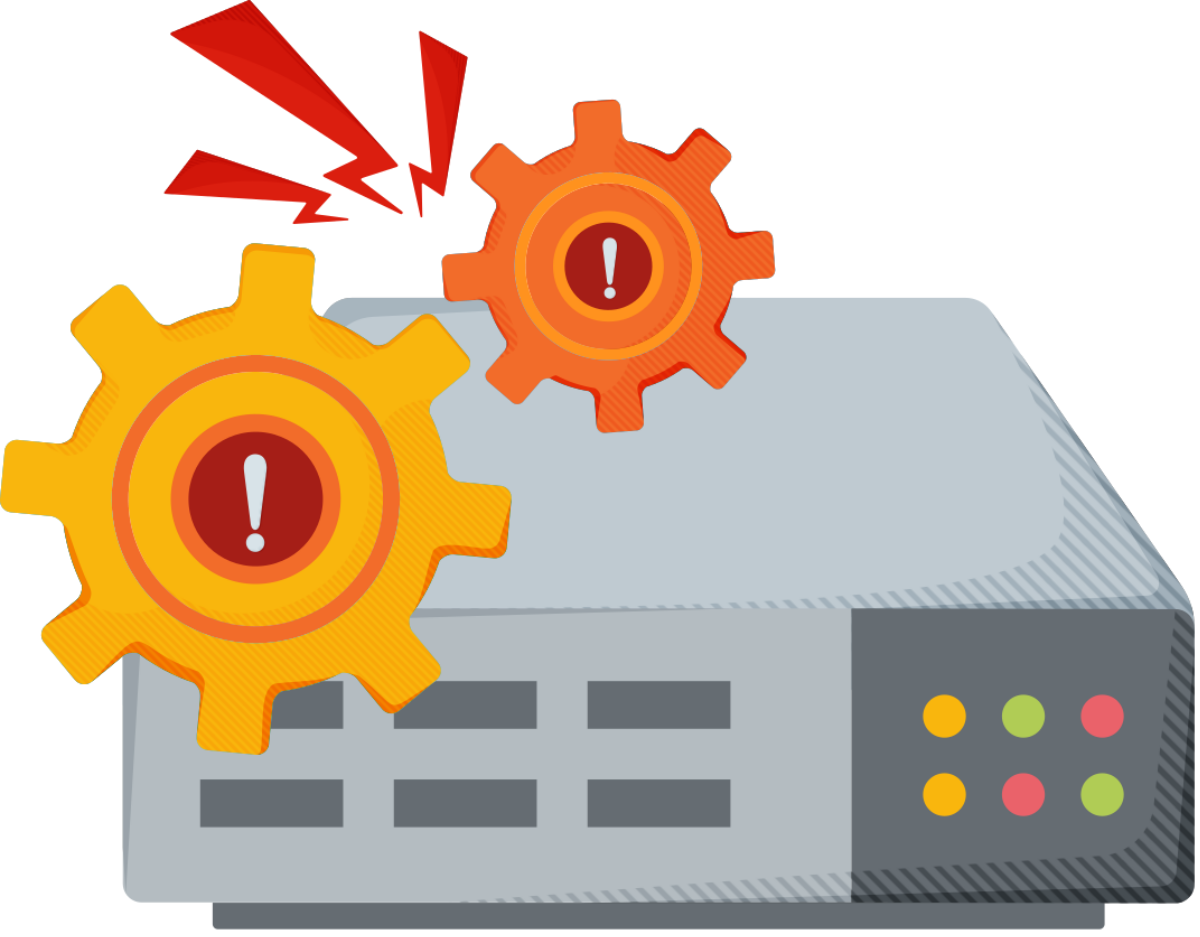
\includegraphics[width=0.25\textwidth]{Images/chapter_13/section_6310983387840512/6291987840237568.png}
 
\end{figure}

When one of the services goes down, it can be the reason for other services to crash, and as a result, the application is unavailable to users. If we don't know what went wrong early, it could take us a lot of time and effort to debug the system manually. Moreover , for larger services, we need to ensure that our services are working within our agreed service-level agreements. We need to catch important trends and signals of impending failures as early warnings so that any concerns or issues can be addressed.\\
\strut \\
Monitoring helps in analyzing such complex infrastructure where something is constantly failing. Monitoring distributed systems entails gathering, interpreting, and displaying data about the interactions between processes that are running at the same time. It assists in debugging, testing, performance evaluation, and having a bird's-eye view over multiple services.

\subsection{How will we design a distributed monitoring system?}\label{I72dScBJatbw98ZmVQ3no}
\\
We've divided the distributed monitoring system design into the following chapters and lessons:

\begin{enumerate}
\item
\protect\phantomsection\label{pqA2-6yxSM_c0uk-Ptog5}
\textbf{Distributed Monitoring}

\begin{enumerate}
\item
\href{https://www.educative.io/courses/grokking-the-system-design-interview/introduction-to-distributed-monitoring}{\textbf{Introduction to Distributed Monitoring}}: Learn why monitoring in a distributed system is crucial, how costly downtime is, and the types of monitoring.
\item
\href{https://www.educative.io/courses/grokking-the-system-design-interview/prerequisites-of-a-monitoring-system}{\textbf{Prerequisites for a Monitoring System}}: Explore a few essential concepts about metrics and alerting in a monitoring system.
\end{enumerate}
\item
\protect\phantomsection\label{Jmh98MHsOwhNPkFrJrIZN}
\textbf{Monitoring Server-side Errors}

\begin{enumerate}
\item
\href{https://www.educative.io/courses/grokking-the-system-design-interview/design-of-a-monitoring-system}{\textbf{Designing a Monitoring System}}: Define the requirements and high-level design of the monitoring system.
\item
\href{https://www.educative.io/courses/grokking-the-system-design-interview/detailed-design-of-a-monitoring-system}{\textbf{A Detailed Design of the Monitoring System}}: Go into the details of designing a monitoring system, and explore the components involved.
\item
\href{https://www.educative.io/courses/grokking-the-system-design-interview/visualize-data-in-a-monitoring-system}{\textbf{Visualize Data in a Monitoring System}}: Learn a unique way to visualize an enormous amount of monitoring data.
\end{enumerate}
\item
\protect\phantomsection\label{HIJFCdxYORcc__-hY3ycE}
\textbf{Monitor Client-side Errors}

\begin{enumerate}
\item
\href{https://www.educative.io/courses/grokking-the-system-design-interview/focus-on-client-side-errors-in-a-monitoring-system}{\textbf{Focus on Client-side Errors}}: Get introduced to client-side errors and why it's important to monitor them.
\item
\href{https://www.educative.io/courses/grokking-the-system-design-interview/design-of-a-client-side-monitoring-system}{\textbf{Design a Client-side Monitoring System}}: Learn to design a system that monitors the client-side errors.
\end{enumerate}
\end{enumerate}
\\
In the next lesson, we'll look at why monitoring is essential in a distributed system through an example. We 'll also look at the downtime cost of failures and monitoring types.

% End of section content